% !BIB program = biber
\documentclass[12pt,english,letterpaper]{kuthesis}
\usepackage{times}
\usepackage{amsmath}
\usepackage{geometry}
\geometry{verbose,tmargin=1in,bmargin=1in,lmargin=1in,rmargin=1in}
\setcounter{secnumdepth}{3}
\setcounter{tocdepth}{3}
\usepackage{color}
\usepackage{babel}
\usepackage{csquotes}
\usepackage{url}
\usepackage{subfig}
\usepackage{graphicx}
\usepackage{setspace}
\usepackage{esint}
\usepackage{amssymb}
\graphicspath{ {./images/} }
\usepackage{xcolor}
\usepackage{slashed}
\usepackage[natbib=true, backend=biber, style=apa,]{biblatex}
\addbibresource{Biblio/allcites.bib}
\usepackage{enumitem}
\usepackage{makecell}
\usepackage{enumitem}
\usepackage{appendix}
\usepackage[acronym]{glossaries}
\setlistdepth{20}
\renewlist{itemize}{itemize}{20}

%%%%%%%%%%%%%%%%%%%%%%%%%%%%%%%%%%%%%%%%%%%%%%%%%%%%%%%%%%%%%%%%%%%%

\doublespacing
\usepackage[unicode=true,
 bookmarks=true,bookmarksnumbered=false,bookmarksopen=false,
 breaklinks=true,pdfborder={0 0 0},pdfborderstyle={},backref=false,colorlinks=true]
 {hyperref}
\hypersetup{pdftitle={University of Kansas Thesis Template},
 pdfauthor={Anonymous},
 pdfsubject={A Thesis},
 urlcolor={black},citecolor={black},allcolors={black}}

\makeatletter

%%%%%%%%%%%%%%%%%%%%%%%%%%%%%% LyX specific LaTeX commands.

\providecommand{\LyX}{\texorpdfstring%
  {L\kern-.1667em\lower.25em\hbox{Y}\kern-.125emX\@}
  {LyX}}
%% Because html converters don't know tabularnewline
\providecommand{\tabularnewline}{\\}

%%%%%%%%%%%%%%%%%%%%%%%%%%%%%% User specified LaTeX commands.

%used to align decimals in tables according to APA style
\usepackage{dcolumn}
\usepackage{booktabs}

\author{Athena Harris}
\title{The Title is Not Dog Treats}
\date{2026}

\priorcreds
{Bachelors of Science in Computer Science, Kansas University, 2024}
{Bachelors of Science in Mathematics, Kansas University, 2024}

% Previous degree entries can be removed or added as needed
% It is also acceptable to delete \priorcreds if the title page becomes too crowded

\dept{Your Department}
\degreetitle{Your Degree}

\papertype{Thesis/Dissertation} % Chose whether it is a Thesis or a Dissertation

\committee{Perry Alexander}{Member 2}{Member 3}{Member 4}{Member 5}{}{} % List the names of your committee members in the brackets

%\committee{Member 1}{Member 2}{Member 3}{Member 4}{Member 5}{}{} % List the names of your committee members in the brackets

\role{Chair:}{}{}{}{}{}{} % List your chair after the "Chair:", e.g., {Chair: John Doe}

% If you have co-chairs, replace the above line with the following and fill it out accordingly:
%\role{Co-Chair:}{Co-Chair:}{}{}{}{}{}

\@printd@testrue
\datedefended{MM DD, YYYY} % This is the date your defended your work

\dateapproved{MM DD, YYYY} % This is the date your work was accepted

\@ifundefined{showcaptionsetup}{}{%
 \PassOptionsToPackage{caption=false}{subfig}}
\usepackage{subfig}
\makeatother

\begin{document}

\maketitle

% The abstract should serve a more organizational purpose. It is a summary of the
% work that a non-expert should be able to read and parse.
% [Introduce Area of study]. [Existing work in area].
% [Introduce work]... [Discuss how it works]... [Discuss results]...
\begin{abstract}

Formal verification is a useful tool in guaranteeing the security and behavior of programs. This is increasingly true as the amount of LLM generated
code continues to rise. However even simple projects can be labor intensive to verify, thus verification see's little use in practice. Existing methods
have either used program synthesis algorithms or LLM's to automate verification. We continue this work with {NotDogTreats} an LLM based proof synthesizer
for Verus which iteratively attempts to construct proofs utilizing prompts containing relevant information about the problem. This consists of tracking 
and ranking information in the local context and providing only the relevant information to the LLM. The process then iteratively attempts to solve 

\end{abstract}

\longstyle

\begin{acknowledgements}

This is where you will insert you acknowledgements. Usually in this section, students will mention their thesis/dissertation chair and committee, any research associates, their friends, and their family members. But who you thank is ultimately up to you.

\end{acknowledgements}

\tableofcontents{}
\listoffigures
\addcontentsline{toc}{chapter}{List of Figures}
\listoftables
\addcontentsline{toc}{chapter}{List of Tables}

\printglossary[title=Abbreviations, style=long,nonumberlist, type=\acronymtype]

\chapter{Introduction} %This is an example title name

\begin{chapterabstract}

This is where you will insert your chapter abstract, which funcitons as a concise, self-contained summary of your chapter.

%Note that chapter abstracts are not required by KU. If your committee feels like you don't need an abstract for each chapter, simply don't include the \begin{chapterabstract} and \end{chapterabstract} commands in each chapter .tex file.

\end{chapterabstract}

%%%%%%%%%%%%%%%%%%%%%%%%%%%%%%%%%%%%%%%%%%%%%%%%%%%%%%%%%%%%%%%%%%%%%%%%%%%%%%%%%%%%%%%%%%
%%%%%%%%%%%%%%%%%%%%%%%%%%%%%%%%%%%%%%%%%%%%%%%%%%%%%%%%%%%%%%%%%%%%%%%%%%%%%%%%%%%%%%%%%%


% 

\section{Overview}
[What is Formal Methods and its significance?] The desire for high availability and secure software has only grown as we continue to rely on computers for critically important functions. Whether that be 
for banking services, pacemaker devices, or AWS a service which hosts [stupid amount of money] in business every second. For any of these cases even minor malfunctions could have significant consequences.
Thus one might be interested in guaranteeing correct behavior for these systems. This is the goal of formal methods where we can formally prove properties about a program via [math...]. However formal 
methods has seen little use in practical applications as the process is unfamiliar to the typical programmer and time-intensive. [Reference a large formally verified program like C compiler project?]. 
[Introduce automated proof tools].

[Discuss past work in proof automation, then the rise of LLM based tools]

[Introduce our work in this field].

Type out the content of your subsection here. What follows is an example APA 7th citation \citep{Met78}. Note also \citet{Met78b} but \citet{Met78c}. You can adjust citational information by editing the allcites.bib file, included in this package.

\section{Background?}
Discuss formal methods and proof synthesis. What someone might need to know to understand this paper, How did the field develop to where we are today, and 
the significance of the field.

\chapter{Literature Review} %This is an example title name

\begin{chapterabstract}

This is where you will insert your chapter abstract, which funcitons as a concise, self-contained summary of your chapter.

%Note that chapter abstracts are not required by KU. If your committee feels like you don't need an abstract for each chapter, simply don't include the \begin{chapterabstract} and \end{chapterabstract} commands in each chapter .tex file.

\end{chapterabstract}

%%%%%%%%%%%%%%%%%%%%%%%%%%%%%%%%%%%%%%%%%%%%%%%%%%%%%%%%%%%%%%%%%%%%%%%%%%%%%%%%%%%%%%%%%%
%%%%%%%%%%%%%%%%%%%%%%%%%%%%%%%%%%%%%%%%%%%%%%%%%%%%%%%%%%%%%%%%%%%%%%%%%%%%%%%%%%%%%%%%%%

\section{Name of Subsection}
Type out the content of your subsection here \citep{Einstein:1933gu}. Delete or duplicate as necessary. Note that you can also refer to figures in the text like this: see figure \ref{sample-image_PD}.

\begin{figure}[h]
\caption{Insert figure caption here}
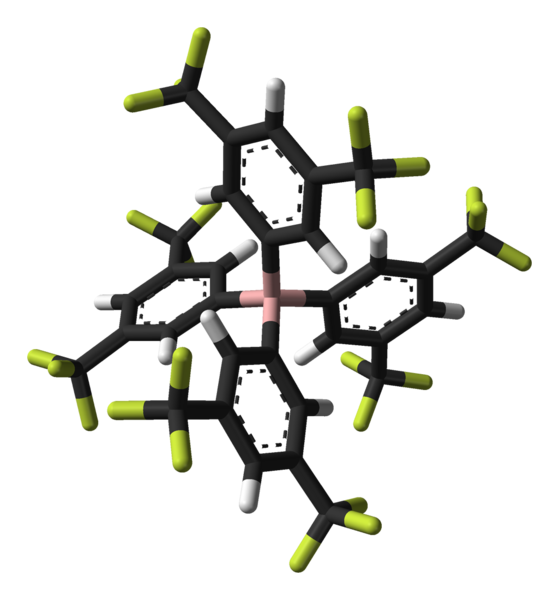
\includegraphics[scale=0.5]{sample-image_PD}
\label{sample-image_PD}
\centering
\end{figure}

%Image courtesy of https://commons.wikimedia.org/wiki/File:BArF-3D-sticks.png

\subsection{Name of Third-Level Subsection}
Here is an example of a third-level subsection. Delete or duplicate as necessary.

\subsubsection{Name of Fourth-Level Subsection}
Here is another example of a fourth-level subsection. Delete or duplicate as necessary.
\chapter{Methodology} %This is an example title name

\begin{chapterabstract}

This is where you will insert your chapter abstract, which funcitons as a concise, self-contained summary of your chapter.

%Note that chapter abstracts are not required by KU. If your committee feels like you don't need an abstract for each chapter, simply don't include the \begin{chapterabstract} and \end{chapterabstract} commands in each chapter .tex file.

\end{chapterabstract}

%%%%%%%%%%%%%%%%%%%%%%%%%%%%%%%%%%%%%%%%%%%%%%%%%%%%%%%%%%%%%%%%%%%%%%%%%%%%%%%%%%%%%%%%%%
%%%%%%%%%%%%%%%%%%%%%%%%%%%%%%%%%%%%%%%%%%%%%%%%%%%%%%%%%%%%%%%%%%%%%%%%%%%%%%%%%%%%%%%%%%

\section{Name of Subsection}
Type out the content of your subsection here. Here's another citation example \citep{Lit96,Wel03,Met78}. And here is an example equation:

\begin{equation}
    \label{eq:iceberg_draft_estimate}
    D = 2.91L{^{0.71}}
\end{equation}

\section{Name of Subsection}
Here is another example of a chapter subsection. Delete or duplicate as necessary.

\subsection{Name of Third-Level Subsection}
Here is another example of a third-level subsection. Delete or duplicate as necessary.

\subsubsection{Name of Fourth-Level Subsection}
Here is another example of a fourth-level subsection. Delete or duplicate as necessary.
\chapter{Findings} %This is an example title name

\begin{chapterabstract}

This is where you will insert your chapter abstract, which funcitons as a concise, self-contained summary of your chapter.

%Note that chapter abstracts are not required by KU. If your committee feels like you don't need an abstract for each chapter, simply don't include the \begin{chapterabstract} and \end{chapterabstract} commands in each chapter .tex file.

\end{chapterabstract}

%%%%%%%%%%%%%%%%%%%%%%%%%%%%%%%%%%%%%%%%%%%%%%%%%%%%%%%%%%%%%%%%%%%%%%%%%%%%%%%%%%%%%%%%%%
%%%%%%%%%%%%%%%%%%%%%%%%%%%%%%%%%%%%%%%%%%%%%%%%%%%%%%%%%%%%%%%%%%%%%%%%%%%%%%%%%%%%%%%%%%

\section{Name of Subsection}
Type out the content of your subsection here. Here's another citation \citep{Einstein:1933gu,Tho98w}. What follows is an example table:

\begin{table}[h]
\caption{Insert table caption here} % title of Table
\centering % used for centering table
\begin{tabular}{c c c c c} % centered columns (5 columns)
\hline\hline %inserts double horizontal lines
Set & Test 1 & Test 2 & Test 3 & Test 4 \\ [0.5ex] % inserts table
%heading
\hline % inserts single horizontal line
1 & 50 & 34 & 837 & 970 \\ % inserting body of the table
2 & 47 & 877 & 34 & 230 \\
3 & 5 & 31 & 25 & 415 \\
4 & 35 & 27 & 144 & 2356 \\
5 & 45 & 300 & 556 & 389 \\ [1ex] % [1ex] adds vertical space
\hline %inserts single line
\end{tabular}
\label{table_example_1:nonlin} % is used to refer to this table in the text
\end{table}

And just to be safe, here is another example of a table:

\begin{table}[h]
\caption{Insert table caption here} 
\centering 
\begin{tabular}{c c c c c c} 
\hline\hline 
Experiment & Batch A & Batch B & Batch C & Batch D & Batch E \\ [0.5ex] 
\hline 
5 & 7 & 5 & 3 & 7 & 2 \\
8 & 9 & 8 & 2 & 1 & 9 \\
3 & 2 & 1 & 9 & 6 & 6 \\
2 & 2 & 8 & 1 & 4 & 9 \\ [1ex] 
\hline 
\end{tabular}
\label{table_example_2:nonlin}
\end{table}

%The above table based on the one from "Creating Tables with LaTeX" (https://web.archive.org/web/20090306042457/http://www1.maths.leeds.ac.uk/latex/TableHelp1.pdf)

You can also refer to tables in the text like this: see tables \ref{table_example_1:nonlin} and \ref{table_example_2:nonlin}.

\section{Name of Subsection}
Here is another example of a chapter subsection. Delete or duplicate as necessary.

\subsection{Name of Third-Level Subsection}
Here is another example of a third-level subsection. Delete or duplicate as necessary.

\subsubsection{Name of Fourth-Level Subsection}
Here is another example of a fourth-level subsection. Delete or duplicate as necessary.
\chapter{Conclusion} %This is an example title name

\begin{chapterabstract}

This is where you will insert your chapter abstract, which funcitons as a concise, self-contained summary of your chapter.

%Note that chapter abstracts are not required by KU. If your committee feels like you don't need an abstract for each chapter, simply don't include the \begin{chapterabstract} and \end{chapterabstract} commands in each chapter .tex file.

\end{chapterabstract}

%%%%%%%%%%%%%%%%%%%%%%%%%%%%%%%%%%%%%%%%%%%%%%%%%%%%%%%%%%%%%%%%%%%%%%%%%%%%%%%%%%%%%%%%%%
%%%%%%%%%%%%%%%%%%%%%%%%%%%%%%%%%%%%%%%%%%%%%%%%%%%%%%%%%%%%%%%%%%%%%%%%%%%%%%%%%%%%%%%%%%

\section{Name of Subsection}
Type out the content of your subsection here. Delete or duplicate as necessary.

\section{Name of Subsection}
Here is another example of a chapter subsection. Delete or duplicate as necessary.

\subsection{Name of Third-Level Subsection}
Here is another example of a third-level subsection. Delete or duplicate as necessary.

\subsubsection{Name of Fourth-Level Subsection}
Here is another example of a fourth-level subsection. Delete or duplicate as necessary.

% If you need to additional chapters, simply remove the "%" at the start of the necessary lines that follow:

%\include{chapters/ch6}
%\include{chapters/ch7}
%\include{chapters/ch8}
%\include{chapters/ch9}
%\include{chapters/ch10}

% Make sure that a .tex file for each additional chapter can be found in the "chapters" folder

\printbibliography[title=References,heading=bibintoc]

\appendix
\chapter{Title of Appendix} %This is an example title name

\section{Name of Subsection}
This is an example of an appendix. You can put citations here \citep{Met78}, as well as figures:

\begin{figure}[h]
\caption{Insert figure caption here}
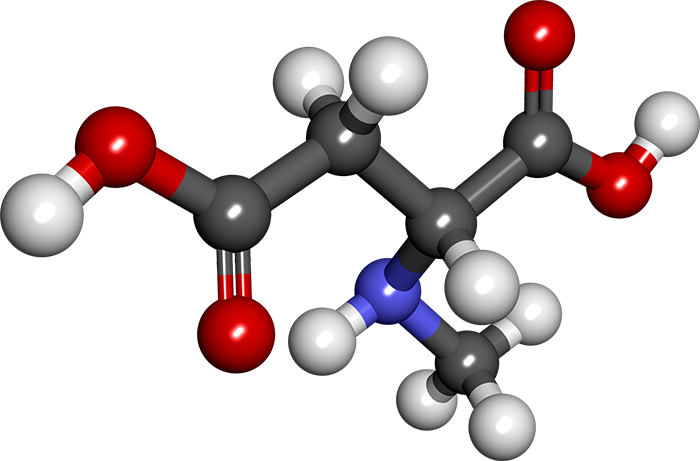
\includegraphics[scale=1]{sample-image_NMDA}
\label{sample-image_NMDA}
\centering
\end{figure}

%Image courtesy of https://commons.wikimedia.org/wiki/File:NMDA2.png

\section{Name of Subsection}
Here is another example of an appendix subsection. Delete or duplicate as necessary.

\subsection{Name of Third-Level Subsection}
Here is another example of a third-level appendix subsection. Delete or duplicate as necessary.

\subsubsection{Name of Fourth-Level Subsection}
Here is another example of a fourth-level appendix subsection. Delete or duplicate as necessary.
\chapter{Title of Appendix} %This is an example title name

\section{Name of Subsection}
This is an example of an appendix. Just like chapters, you can also include tables in appendices:

\begin{table}[h]
\caption{Insert table caption here} 
\centering 
\begin{tabular}{c c c c c c} 
\hline\hline 
Experiment & Batch A & Batch B & Batch C & Batch D & Batch E \\ [0.5ex] 
\hline 
6 & 9 & 5 & 3 & 7 & 2 \\
8 & 3 & 8 & 2 & 1 & 9 \\
9 & 7 & 1 & 9 & 6 & 6 \\
9 & 4 & 8 & 1 & 4 & 9 \\ [1ex] 
\hline 
\end{tabular}
\label{table_example_3:nonlin}
\end{table}

\section{Name of Subsection}
Here is another example of an appendix subsection. Delete or duplicate as necessary.

\subsection{Name of Third-Level Subsection}
Here is another example of a third-level appendix subsection. Delete or duplicate as necessary.

\subsubsection{Name of Fourth-Level Subsection}
Here is another example of a fourth-level appendix subsection. Delete or duplicate as necessary.

%If you need to additional appendices, simply remove the "%" at the start of the necessary lines that follow:

%\include{chapters/AppendixC}
%\include{chapters/AppendixD}
%\include{chapters/AppendixE}
%\include{chapters/AppendixF}
%\include{chapters/AppendixG}
%\include{chapters/AppendixH}

% Make sure that a .tex file for each additional appendix can be found in the "chapters" folder

\end{document}